\section{Content Background}\label{content}

In the following, we will consider fault-proneness as already mentioned, but from a restricted point of view, in an object-oriented context. Many software systems in use are based on object-oriented design. This means that data and program code are encapsulated in reusable objects. Everything is based on the communication of objects. For this purpose, classes, interfaces and methods, as well as attributes are declared and thus serve to represent states. This structure alone protects against fault-proneness, since the code is reusable and thus the programming effort is reduced. Therefore, object orientation in itself offers advantages for maintainability and reusability. Thus, fewer errors occur \cite{fichman1993adoption, lanza2002beyond}. 

In the object oriented context there are a few constructs like class, coupling, cohesion, inheritance, information hiding and polymorphism, which also influence the fault-proneness. Examples of languages that program object-oriented are C\#, C++ or Java.
One of the most common aspects incorporated into metrics is that of coupling, which refers to the degree of direct knowledge that one element has of another. The degree of interconnectedness of the whole system is a key element in the software development, for example it is important how big the effect of changing one attribute of one class has on all others and especially how many.
The coupling of the classes in the system plays a central role in the effects of software faults.
To give a short introduction in object orientation and the relation between its properties, it is shown in figure \ref{fig0}, that invoking methods and accessing attributes is the basic principle of communication of these software systems, which means that faults can occur here depending on the frequency of use. In how far the interaction of the individual components are connected with the fault-proneness metrics, is described in the metrics chapter \ref{analysis} more near.

\begin{figure}[htbp]
	\centerline{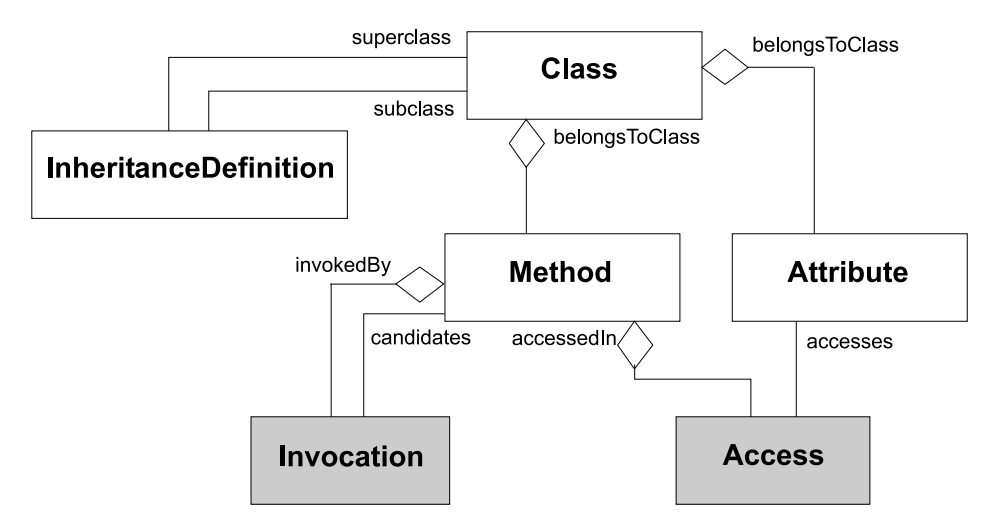
\includegraphics[width=0.5\textwidth]{pictures/oodesign.png}}
	\caption{A meta model for main object-oriented concepts \cite{lanza2002beyond}.}
	\label{fig0}
\end{figure}

But why should a programmer actually pay attention to fault-proneness at all? The accurate prediction of where bugs are more likely to occur in the code can help manage efforts in testing, reduce costs, and improve the quality of the software. For different programming paradigms and programming constructs different rules apply which must be considered in relation to fault-proneness.  The restriction on object orientation is to facilitate the understanding. In addition many principles are contained, which are taken up in other programming concepts again. Thus some conclusions which are drawn here are also differently realizable and applicable to other software concepts.

In terms of fault-proneness, other quality characteristics that must not be forgotten also play a role like reliability, correctness, completeness, maintainability, as some are dependent on each other in terms of time. For example, software may not be reliable or correct if faults occur frequently that cause the software to become unusable.

When software errors are made, it is often not only tedious to find the programming error, but also expensive. In large systems that are used by many people every day, a small error can cost millions. When software errors are made, it is often not only tedious to find the programming error, but also expensive. In large systems that are used by many people every day, a small error can cost millions. A common misconception is that fault-proneness should only be considered at the end of the software development process. Especially at the beginning of the development you should build the software architecture in a way that it is less fault-prone. Changes in the architecture are always more expensive later. In addition, even before the programming itself begins, attention should be paid in the planning to various concepts and metrics, which are shown below.

- to what extent can you do analysis now and what should you consider when developing object-oriented

- research background: summary of interpretation of previous research and what this paper is about depending on the research